\documentclass[10pt,landscape,a4paper]{article}
\usepackage[utf8]{inputenc}
\usepackage[ngerman]{babel}
\usepackage{ctex}
\usepackage{graphicx}
\usepackage{pifont}
\usepackage{tabularx}
\usepackage[T1]{fontenc}
\usepackage{graphics}
\usepackage{enumitem}
\usepackage{tikz}
\usetikzlibrary{shapes,positioning,arrows,fit,calc,graphs,graphs.standard}
\usepackage[nosf]{kpfonts}
\usepackage[t1]{sourcesanspro}
\usepackage{multicol}
\usepackage{wrapfig}
\usepackage[top=2mm,bottom=2mm,left=2mm,right=2mm]{geometry}
\usepackage[framemethod=tikz]{mdframed}
\usepackage{microtype}
\usepackage{pdfpages}
\usepackage{cancel}

\let\bar\overline
\newfontface\CJKfont{SimSun}
\setlength{\columnsep}{10pt} % 设置栏间距
\setlength{\columnseprule}{0.2pt}
\setlength{\parskip}{2pt}
\setlist{topsep=0em,itemsep=-0.5em, labelsep=0em, leftmargin=1.5em}

\sloppy
\begin{document}
%\definecolor{myblue}{cmyk}{1,.72,0,.38}

\def\firstcircle{(0,0) circle (1.5cm)}
\def\secondcircle{(0:2cm) circle (1.5cm)}

\newenvironment{figurehere}
    {\def\@captype{figure}}
    {}
\makeatother

%\colorlet{circle edge}{myblue}
%\colorlet{circle area}{myblue!5}

\tikzset{filled/.style={fill=circle area, draw=circle edge, thick},
    outline/.style={draw=circle edge, thick}}
    
\pgfdeclarelayer{background}
\pgfsetlayers{background,main}

%\everymath\expandafter{\the\everymath \color{myblue}}
%\everydisplay\expandafter{\the\everydisplay \color{myblue}}

\renewcommand{\baselinestretch}{.8}
\pagestyle{empty}

\global\mdfdefinestyle{header}{%
linecolor=gray,linewidth=1pt,%
leftmargin=0mm,rightmargin=0mm,skipbelow=0mm,skipabove=0mm,
}

\newcommand{\header}{
\begin{mdframed}[style=header]
\footnotesize
\sffamily
Hilfszettel zur Klausur\\
von~Tim~S.,~Seite~\thepage~von~2
\end{mdframed}
}

\makeatletter % Author: https://tex.stackexchange.com/questions/218587/how-to-set-one-header-for-each-page-using-multicols
\renewcommand{\section}{\@startsection{section}{1}{0mm}%
                                {.2ex}%
                                {.2ex}%x
                                {\sffamily\scriptsize\bfseries}}
\renewcommand{\subsection}{\@startsection{subsection}{1}{0mm}%
                                {.2ex}%
                                {.2ex}%x
                                {\sffamily\scriptsize\bfseries}}




\makeatother
\setlength{\parindent}{0pt}
\scriptsize
\begin{multicols*}{6}
\centerline{\textbf{离散数学期末知识点汇总~~$2025.1$}}
\fontsize{6pt}{7pt}
\section*{命题、联结词与命题公式}

\textbf{命题}:非真即假/可明确判真假的陈述句\\
·\textbf{悖论}:[我正在撒谎]既不为真也不为假\\
· [长方形是正方形]既可为真也可为假

\textbf{真值}:命题的判断结果,只取真或假两个值

\textbf{真命题/假命题}:真值为真/假的命题

\textbf{命题符号化}:将命题抽象为取值为0or1的$p$,$q$...

\textbf{简单命题(原子命题)}:不能被分解成更简单的命题的命题

\textbf{复合命题}:由简单命题通过联结词联结而成的命题

·其真假完全由构成它的简单命题的真假决定

·简单命题和复合命题的划分是相对的

\textbf{否定式}:复合命题“非$p$”称作$p$的否定式,$\neg p$

\textbf{否定联结词}:$\neg$,规定$\neg p$为真当且仅当$p$为假

\textbf{合取式}:复合命题“$p$并且$q$”称为$p$与$q$的合取式,记作$p \wedge q$

\textbf{合取联结词}:$\wedge$,规定$p \wedge q$为真当且仅当$p$与$q$同时为真

\textbf{析取式}:复合命题“$p$或$q$”称作$p$与$q$的析取式,记作$p \vee q$

\textbf{析取联结词}:$\vee$,规定$p \vee q$为假当且仅当$p$与$q$同时为假

·\textbf{相容或与相斥或}:$\vee$与$\bar{\vee}$, $\bar{\vee}$为真要满足$p, q$不同时为真;不能看见$p$或$q$就转化为$p \vee q$

\textbf{蕴涵式}:复合命题“如果$p$,则$q$”称为$p$与$q$的蕴涵式,记作$p \rightarrow q$,并称$p$是前件,$q$是后件

·例子:如果$p$则$q$;$q$每当$p$;$p$仅当$q$;只有$q$才$p$;除非$q$才$p$;除非$q$,否则$\lnot p$

\textbf{蕴涵联结词}:$\rightarrow$,规定$p \rightarrow q$为假当且仅当$p$为真而$q$为假($p \le q$)

\textbf{等价式}:复合命题“$p$当且仅当$q$”称作$p$与$q$的等价式,记作$p \leftrightarrow q$

\textbf{等价联结词}:$\leftrightarrow$,规定$p \leftrightarrow q$为真当且仅当$p$与$q$同时为真或同时为假

\textbf{命题常量}:一个特定的命题,真值确定

\textbf{命题变量/项/元}:一个没有赋予具体内容的命题,真值可变

\textbf{命题公式(命题形式)}:由命题变元和联结词按以下规则组成的符号串\\
1.任何命题变元都是命题公式,称为原子命题公式\\
2.如果$A$是命题公式,则$\lnot A$也是命题公式\\
3.如果$A$、$B$是命题公式,则$(A \vee B)$、$(A \wedge B)$、$(A \rightarrow B)$和$(A \leftrightarrow B)$都是命题公式\\
只有有限次地应用(1)—(3)构成的符号串才是命题公式\\
命题公式定义是归纳定义,而不是循环定义,(1)是奠基,(2)、(3)是归纳步骤

·公式中的0, 1看作可看作$(A \wedge (\lnot A))$、$(A \vee (\lnot A))$

\textbf{约定运算顺序}

省略命题公式最外层括号;$\lnot$的优先级高于其它的联结词,只作用于紧随其后的命题变元;相同联结词可以省略括号;优先级:(否定) > (合取、析取) > (蕴涵、等价)

\textbf{赋值(解释)}:设$p_1, p_2, \ldots, p_n$是出现在命题公式$A$中的所有命题变元,对序列$p_1, p_2, \ldots, p_n$指定的的任一真值序列,称为对$A$的一个赋值

\textbf{成真/假赋值}:若$p_1, p_2, \ldots, p_n$的一个赋值使$A$为真/假,则称此赋值为$A$的一个成真/假赋值

\textbf{重言式(永真式)/矛盾式(永假式)}:$A$关于其中出现的命题变元的所有赋值均为成真/假赋值

\textbf{可满足式}:$A$对于其中出现的命题变元的某个赋值为成真赋值

\textbf{哑元}:未出现在$A$中的命题变元,$A$取值与哑元取值无关

\section*{等值式与范式}

\textbf{等值式}:若$A, B$构成的等价式$A \leftrightarrow B$为重言式,则称$A$与$B$等值,记作$A \Leftrightarrow B$,并称$A \Leftrightarrow B$是等值式;等值是一种等价关系

\textbf{文字}:命题变项及其否定的统称

\textbf{简单析/合取式}:仅由有限个文字构成的析/合取式

\textbf{范式}:由有限个简单合/析取式的\textbf{析/合}取构成的命题公式称作\textbf{析/合}取范式;析取范式与合取范式统称作范式

·简单合(析)取式既是析取范式又是合取范式

\textbf{极小/大项}:以含$p, q, r$的情况为例\\
·$m_1 = \lnot p \wedge \lnot q \wedge r$(下标=成真赋值)\\
·$M_1 = p \vee q \vee \lnot r$(下标=成假赋值)

\textbf{主析/合取范式}:所有简单合/析取式都是极小/大项的析/合取范式

\textbf{n元真值函数}:$F:\{0,1\}^n \rightarrow \{0,1\}$

\textbf{联结词的完备集S}:仅由$S$中的联结词构成的公式可表示所有真值函数

\textbf{与非、或非}:$\uparrow$表示与非,$\downarrow$表示或非

\section*{命题逻辑推理}
	
\textbf{推理形式}:由前提 $\alpha_1$, $\alpha_2$, $\cdots$, $\alpha_n$ 推出结论 $\beta$

\textbf{推理正确(有效)}:如果对 $\alpha_1$, $\cdots, \alpha_n$, $\beta$ 中出现的命题变元的任意赋值,若 $\alpha_1 \land \alpha_2 \land \cdots \land \alpha_n$ 为假,或若 $\alpha_1 \land \alpha_2 \land \cdots \land \alpha_n$ 为真时 $\beta$ 亦真,则称推理 "$\alpha_1$, $\alpha_2$, $\cdots$, $\alpha_n$ 推出 $\beta$" 有效,否则是不合理(无效)的。

·注:若出现\textbf{前提为真结论为假}的情况则推理无效!

\textbf{逻辑蕴涵}$\Rightarrow$: 前提:$\alpha_1$, $\alpha_2$, $\cdots$, $\alpha_n$ 结论:$\beta$ 推理正确记为 $\alpha_1 \land \alpha_2 \land \cdots \land \alpha_n \Rightarrow \beta$

·$A \rightarrow B$ 是命题公式,$A \Rightarrow B$ 表示两个命题公式之间的逻辑蕴涵关系

\textbf{自然推理系统P}:\\
·字母表:命题变元、联结词、括号逗号\\
·命题公式:(见上)\\
·推理规则:(见定理)

\section*{一阶谓词逻辑}

\textbf{个体}:独立存在的客体\\
·个体常元:表示具体事物,$a, b, c, \ldots$\\
·个体变元:抽象事物(不确定具体哪个) $x, y, z, \ldots$

\textbf{个体域}:个体变元的取值范围\\
·全总个体域:由宇宙间一切事物组成的个体域

\textbf{谓词}:表示个体性质或彼此之间关系$F, G, H, \ldots$\\
·谓词常元:表示具体性质或关系\\
·谓词变元:表示抽象的或泛指的性质或关系

\textbf{n元谓词}:含 $n$ 个【个体变元】的谓词,是定义在个体域上,值域为 $\{0,1\}$ 的 $n$ 元函数\\
·一元谓词:表示事物的性质\\
·多元谓词:表示事物之间的关系\\
·0元谓词:不含个体变元的谓词,就是命题常项或命题变项

注:将 $n$ 元谓词中的个体变元都用个体域中具体的个体取代后,就成为一个命题

\textbf{量词}:表示数量的词\\
\textbf{全称量词 $\forall$}:自然语言中“所有的”、“一切的”、“任意的”、“每一个”、“都”等的统称。 $\forall x$ 个体域中的所有个体; $\forall x F(x)$ 个体域里的所有 $x$ 都有性质 $F$\\
\textbf{存在量词 $\exists$}:自然语言中“有一个”、“至少有一个”、“存在着”、“有的”等的统称。 $\exists x$ 存在个体域里的 $x$; $\exists x F(x)$ 在个体域里存在 $x$ 具有性质 $F$

\textbf{有限域下的公示表示法}(无穷集下无)

·$\forall x P(x) = P(1) \land P(2) \land \ldots \land P(k)$:对任意的 $x$,$P(x)$ 均成立,合取联结词的推广

·$\exists x P(x) = P(1) \lor P(2) \lor \ldots \lor P(k)$:有一个 $x$ 使得 $P(x)$ 成立,析取联结词的推广

\textbf{特性谓词 $M(x)$}:用于将个体变元局限在满足该谓词代表的性质或关系的范围之内

\textbf{命题符号化}应注意以下几点:

·两个基本公式:$\forall x (M(x) \rightarrow F(x))$,个体域中所有有性质 $M$ 的个体都有性质 $F$;$\exists x (M(x) \land G(x))$,个体域中存在有性质 $M$ 同时有性质 $G$ 的个体

·同一命题在不同个体域中符号化形式可能不同

·同一命题在不同个体域中真值可能不同

·命题中表示性质和关系的谓词,分别符号化为一元和 $n$ 元谓词

·多个量词出现时,仅同类量词可交换顺序

·定理:$(\exists x)(\forall y) P(x,y) \Rightarrow (\forall y)(\exists x) P(x,y)$

\textbf{函数符号}:个体域$D$上,$n$元函数符号$f(x_1, \dots, x_n)$是$D^n\rightarrow D$的函数(与谓词差异在于值域)

\textbf{一阶语言 $\mathcal{L}$ 的字母表}

非逻辑符号:所描述的特定对象中的符号\\
·个体常元:$a, b, c, \ldots, a_{i}, b_{i}, c_{i}, i \geq 1$\\
·函数符号:$f, g, h, \ldots, f_{i}, g_{i}, h_{i}, \ldots, i \geq 1$\\
·谓词符号:$F, G, H, \ldots, F_{i}, G_{i}, H_{i}, i \geq 1$
	
逻辑符号:逻辑系统中的符号\\
·个体变元:$x, y, z, \ldots, x_{i}, y_{i}, z_{i}, \ldots, i \geq 1$\\
·量词符号:$\forall, \exists$\\
·联结词符号:$\neg, \land, \vee, \rightarrow, \leftarrow$\\
·括号与逗号:(), \, 

\textbf{$\mathcal{L}$ 的项}\\
1. 个体常元和个体变元是项\\
2. 若 $\varphi (x_{1}, x_{2}, \ldots, x_{n})$ 是 $n$ 元函数,$t_{1}, t_{2}, \ldots, t_{n}$ 是任意的 $n$ 个项,则 $\varphi (t_{1}, t_{2}, \ldots, t_{n})$ 是项\\
3. 所有的项都是有限次使用 (1), (2) 得到的

\textbf{原子公式}:设 $R(x_1, x_2, \ldots, x_n)$ 是 $\mathcal{L}$ 任意的 $n$ 元谓词,$t_1, t_2, \ldots, t_n$ 是 $\mathcal{L}$ 的任意 $n$ 个项,则称 $R(t_1, t_2, \ldots, t_n)$ 是原子公式

\textbf{定义 $\mathcal{L}$ 的合式公式}\\
1. 原子公式是合式公式\\
2. 若 $A$ 是合式公式,则 $(\neg A)$ 也是合式公式\\
3. 若 $A$, $B$ 是合式公式,则 $(A \land B), (A \vee B), (A \rightarrow B), (A \leftrightarrow B)$ 也是合式公式\\
4. 若 $A$, $B$ 是合式公式,则 $(\forall x)A, (\exists x)A$ 也是合式公式

·项是(复合)个体;(原子)公式是完整的判断

注1:一阶语言中的原子公式取代了命题公式

注2:所有一阶语言中都含有相同的逻辑符号,但所含的非逻辑符号不一定相同

注3:在定义中没有要求个体$x$一定要在$A$中出现,$(\forall x_1)F(x_1,x_2),(\forall x_3)F(x_1,x_2)$都是公式

注4:$L$中至少有一个谓词符号,否则$L$生成的一阶语言中没有公式

\textbf{括号省略规则}\\
1.省略公式最外层的括号\\
2.联结词$\lnot$的优先级高于其他联结词,可以去掉($\neg\alpha$)中的外层括号\\
3.$\forall x, \exists x$优先级高于所有联结词,将$(\forall x)\alpha, (\exists x)\alpha$记作$\forall x \alpha, \exists x \alpha$;$(\forall x_1) \cdots (\forall x_n)\alpha$简记为$\forall x_1 \cdots \forall x_n \alpha$,$(\exists x_1) \cdots (\exists x_n)\alpha$简记为$\exists x_1 \cdots \exists x_n \alpha$

\textbf{辖域}:公式 $\forall x A$ 和 $\exists x A$ 中,称 $x$ 为 \textbf{指导变元},$A$ 为相应量词的 \textbf{辖域}

\textbf{约束出现}:在 $\forall x$ 和 $\exists x$ 的辖域中(包括 $\forall x$ 和 $\exists x$ 中的 $x$),$x$ 的所有出现称为约束出现,$A$ 中不是约束出现的其他变元称为 \textbf{自由出现}

\textbf{约束变元}:设个体变元 $x$ 在公式 $\alpha$ 中出现,若 $x$ 在 $\alpha$ 中的所有出现【均】为约束出现,则称 $x$ 为 $\alpha$ 的约束变元;否则称为\textbf{自由变元}


\textbf{闭式}:设 $A$ 是任意的公式,若 $A$ 中不含自由出现的个体变元,则称 $A$ 为封闭的公式,简称闭式

·要将含 $r$ 个自由出现的个体变元的公式变成闭式,至少需要加上 $r$ 个量词

\textbf{解释与赋值}

·设一阶语言 $\mathcal{L}$ 个体常元集 $\{ a_{i} \}$,函数符号集 $\{ f_{i} \}$,谓词符号集 $\{ F_{i} \}$,$\mathcal{L}$ 的解释 $I$ 由下面 4 部分组成:\\
1. 非空个体域 $D_I$\\
2. 对每一个个体常元 $a_i, \bar{a_{i}} \in D_I$,称作 $a_{i}$ 在 $I$ 中的解释\\
3. 对每一个函数符号 $f_{i}$,设其为 $m$ 元的,$\bar{f_{i}}$ 是 $D_I$ 上的 $m$ 元函数,称作 $\bar{f_{i}}$ 在 $I$ 中的解释\\
4. 对每一个谓词符号 $F_{i}$,设其为 $n$ 元的,$\bar{F_{i}}$ 是一个 $n$ 元谓词,称作 $F_{i}$ 在 $I$ 中的解释

·$I$下的\textbf{赋值} $\sigma$:对每一个【自由出现】的个体变元 $x$ 指定个体域中的一个值 $\sigma(x)$\\
\fontsize{4pt}{5pt}
注1:任何公式在给定的解释和赋值下都是命题\\
注2:闭式在任何解释下都变成命题(无需赋值)

\fontsize{6pt}{7pt}
\textbf{永真式(逻辑有效式)}:无成假解释和赋值\\
\textbf{矛盾式(永假式)}:无成真解释和赋值\\
\textbf{可满足式}:至少有一个成真解释和赋值

\textbf{代换实例}:
设 $A_0$ 是含命题变项 $p_1, p_2, \ldots, p_n$ 的命题公式,$A_1, A_2, \ldots, A_n$ 是 $n$ 个谓词公式,用 $A_i$ 处处代替 $A_0$ 中的 $p_i (1 \leq i \leq n)$,所得公式 $A$ 称为 $A_0$ 的代换实例。例如,$F(x) \rightarrow G(x)$, $\forall x F(x) \rightarrow \exists y G(y)$ 都是 $p \rightarrow q$ 的代换实例

\textbf{等值式}:设 $A, B$ 是一阶逻辑中任意两个公式,若 $A \leftrightarrow B$ 是永真式,则称 $A$ 与 $B$ 等值,记作 $A  \Leftrightarrow B$,并称 $A  \Leftrightarrow B$ 为等值式

\textbf{前束范式}:一阶逻辑公式 $A$ 具 $Q_{1} x_{1} \ldots Q_{k} x_{k} B$ 的形式。其中 $Q_{i} = \forall$ 或 $\exists$,$B$(母式/基式)不含量词

\textbf{推理正确(有效)}:在一阶逻辑中,从前提 $A_1, \ldots, A_k$ 推出结论 $B$ 正确,若 $A_{1} \land \ldots \land A_{k} \rightarrow B$ 为永真式,记作 $A_{1} \land \ldots \land A_{k} \Rightarrow B$,否则称推理不正确

\textbf{自然推理系统 $N_L$}
一阶逻辑自然推理系统包括:\\
1. 字母表:同一阶语言字母表\\
2. 合式公式(谓词公式):(见上)\\
3. 推理规则:(见定理)


\hrule

\section*{等值式与范式定理}

\textbf{交换律} $A \vee B  \Leftrightarrow B \vee A, A \land B  \Leftrightarrow B \land A, A \leftrightarrow B  \Leftrightarrow B \leftrightarrow A$

\textbf{结合律} $(A \vee B) \vee C  \Leftrightarrow A \vee (B \vee C)$, $(A \land B) \land C  \Leftrightarrow A \land (B \land C)$, $(A \leftrightarrow B) \leftrightarrow C  \Leftrightarrow A \leftrightarrow (B \leftrightarrow C)$

\textbf{分配律} $A \rightarrow (B \rightarrow C)  \Leftrightarrow (A \rightarrow B) \rightarrow (A \rightarrow C)$

$A \vee (B \land C)  \Leftrightarrow (A \vee B) \land (A \vee C)$,与或可互换

\textbf{双重否定律} $A  \Leftrightarrow \neg \neg A$

\textbf{德摩根律} $\neg (A \vee B)  \Leftrightarrow \neg A \land \neg B, \neg (A \land B)  \Leftrightarrow \neg A \vee \neg B$

\textbf{幂等律} $A \vee A \Leftrightarrow A, A \land A \Leftrightarrow A, A \rightarrow A \Leftrightarrow 1, A \leftrightarrow A  \Leftrightarrow 1$

\textbf{吸收率} $A \vee (A \land B)  \Leftrightarrow A, A \land (A \vee B)  \Leftrightarrow A$

\textbf{零律} $A \vee 1  \Leftrightarrow 1, A \land 0 \Leftrightarrow 0, A \rightarrow 1 \Leftrightarrow 1, 0 \rightarrow A \Leftrightarrow 1$

\textbf{同一律} $A \vee 0  \Leftrightarrow A, A \land 1  \Leftrightarrow A, A \rightarrow 0  \Leftrightarrow \lnot A, 0 \leftrightarrow A  \Leftrightarrow \lnot A$

\textbf{排中律} $A \vee \neg A  \Leftrightarrow 1$

\textbf{矛盾律} $A \land \neg A  \Leftrightarrow 0$

\textbf{蕴涵等值式} $A \rightarrow B  \Leftrightarrow \neg A \vee B$

\textbf{等价等值式} $A \leftrightarrow B  \Leftrightarrow (A \rightarrow B) \land (B \rightarrow A)$

\textbf{假言易位} $A \rightarrow B  \Leftrightarrow \neg B \rightarrow \neg A$

\textbf{等价否定等值式} $A \leftrightarrow B  \Leftrightarrow \neg A \leftrightarrow \neg B$

\textbf{归谬律} $(A \rightarrow B) \land (A \rightarrow \neg B)  \Leftrightarrow \neg A$

\textbf{其他} $A \rightarrow \neg A  \Leftrightarrow \neg A, \neg A \rightarrow A  \Leftrightarrow A, A \leftrightarrow \neg A  \Leftrightarrow 0$

$A \rightarrow (B \rightarrow C)  \Leftrightarrow (A \land B) \rightarrow C  \Leftrightarrow B \rightarrow (A \rightarrow C)$

$A \leftrightarrow B  \Leftrightarrow (A \land B) \vee (\neg A \land \neg B)  \Leftrightarrow (\neg A \vee B) \land (A \vee \neg B)$

$(A \rightarrow C) \land (B \rightarrow C)  \Leftrightarrow (A \vee B) \rightarrow C$

\textbf{置换规则}:设 $\phi(A)$ 是含公式 $A$ 的公式,用公式 $B$ 置换 $\phi(A)$ 中的 $A$,得公式 $\phi(B)$,如果 $A  \Leftrightarrow B$,则 $\phi(A)  \Leftrightarrow \phi(B)$

\textbf{证明等值式}:真值表法/等值演算

\textbf{证明不等值式}:真值表法/观察出一个不等值的赋值/先等值演算再观察

·一个简单\textbf{析取式是重言式}当且仅当它同时含某个命题变项及它的否定式

·一个简单\textbf{合取式是矛盾式}当且仅当它同时含某个命题变项及它的否定式

·一个析取范式是矛盾式当且仅当它的\textbf{每个简单合取式}都是\textbf{矛盾式}

·一个合取范式是重言式当且仅当它的\textbf{每个简单析取式}都是\textbf{重言式}

\textbf{范式存在定理}:任一命题公式都存在与之等值的析取范式与合取范式

·方法:利用蕴涵等值式和等价等值式消去;利用双重否定式和德摩根率将$\lnot$消去或内移;分配律

\textbf{一些联结词的完备集}:$\{\lnot, \wedge\}, \{\lnot, \vee\}, \{\lnot, \rightarrow\}, \{\uparrow\}, \{\downarrow\}$

·证明:从主析取出发得$\{\lnot, \wedge, \vee\}$,其他通过符号间的表示

·不考虑与非、或非,2元素有3个完备,3元素有6个完备(含$\lnot$即可),4元素有4个完备

\section*{命题逻辑的推理定律}

\textbf{$\Rightarrow$的基本性质}\\
·若 $A \Rightarrow B$,$A$ 为重言式,则 $B$ 也是重言式\\
·若 $A \Rightarrow B$,$B \Rightarrow A$ 同时成立,必有 $A  \Leftrightarrow B$\\
·若 $A \Rightarrow B$,$B \Rightarrow C$,则 $A \Rightarrow C$\\
·若 $A \Rightarrow B$,$A \Rightarrow C$,则 $A \Rightarrow B \land C$\\
·若 $A \Rightarrow C$,$B \Rightarrow C$,则 $A \lor B \Rightarrow C$

\textbf{证明推理公式 $A \Rightarrow B$ 的方法}

·真值表法;直观解释法【关注前提为真结论为假】

·主析取/合取范式法;等值演算法【根据充要条件 $A \rightarrow B$ 为永真式或$A \land \neg B$ 为矛盾式】

·若 $\neg B \Rightarrow \neg A$,则 $A \Rightarrow B$

\textbf{附加律}:$A \Rightarrow (A \vee B)$

\textbf{化简律}:$(A \land B) \Rightarrow A$

\textbf{假言推理}:$(A \rightarrow B) \land A \Rightarrow B$

\textbf{拒取式}:$(A \rightarrow B) \land \neg B \Rightarrow \neg A$

\textbf{析取三段论}:$(A \vee B) \land \neg A \Rightarrow B$, $(A \vee B) \land \neg B \Rightarrow A$

\textbf{假言三段论}:$(A \rightarrow B) \land (B \rightarrow C) \Rightarrow (A \rightarrow C)$

\textbf{等价三段论}:$(A \leftrightarrow B) \land (B \leftrightarrow C) \Rightarrow (A \leftrightarrow C)$

\textbf{构造性二难}:$(A \rightarrow B) \land (C \rightarrow D) \land (A \vee C) \Rightarrow (B \vee D)$

\textbf{构造性二难(特殊形式)}:$(A \rightarrow B) \land (\neg A \rightarrow B) \Rightarrow B$

\textbf{破坏性二难}:$(A \rightarrow B) \land (C \rightarrow D) \land (\neg B \vee \neg D) \Rightarrow (\neg A \vee \neg C)$

\textbf{推理定律 10}:$\neg A \Rightarrow (A \rightarrow B)$;$B \Rightarrow (A \rightarrow B)$;$\neg (A \rightarrow B) \Rightarrow A$;$\neg (A \rightarrow B) \Rightarrow \neg B$

\textbf{推理定律 11}:$(B \rightarrow C) \Rightarrow (A \rightarrow B) \rightarrow (A \rightarrow C)$;$(B \rightarrow C) \Rightarrow (A \vee B) \rightarrow (A \vee C)$

\textbf{利用自然推理系统P构造推理的证明}:

·\textbf{推理规则}:前提引入规则、结论引入规则、置换规则、合取引入规则($A, B \Rightarrow A \land B$)

1.\textbf{直接证明法}

2.\textbf{附加前提证明法}:如果推理的结构有如下形式:$(A_1 \land A_2 \land \ldots \land A_k) \rightarrow (C \rightarrow B)$,则可以将结构改写为:$(A_1 \land A_2 \land \ldots \land A_k \land C) \rightarrow B$[\textbf{附加前提引入}]

3.\textbf{归谬法}:引入结论的否定作为附加前提,若能推出矛盾式,则此推理有效[\textbf{结论否定引入}]

4.\textbf{消解证明法}:把【结论的否定】及【前提】都化成合取范式,以这些合取范式中的【简单析取式】为前提,仅用归结规则规则构造证明推出0

·归结规则:$(A \vee B) \land (\lnot A \vee C) \Rightarrow B \vee C$

\section*{一阶谓词逻辑等值式}

1.命题逻辑等值式的代换实例都是一阶逻辑的等值式

2.1\textbf{量词否定等值式} $A(x)$ 是含 $x$ 自由出现的公式:
\begin{enumerate}
	\item $\neg \forall x A(x)  \Leftrightarrow \exists x \neg A(x)$
	\item $\neg \exists x A(x)  \Leftrightarrow \forall x \neg A(x)$
\end{enumerate}

2.2\textbf{量词辖域收缩与扩张等值式}:$A(x)$ 是含 $x$ 自由出现的公式;$B$ 中不含 $x$ 的自由出现:
\begin{enumerate}
	\item$\forall x (A(x) \vee B) \Leftrightarrow \forall x A(x) \vee B$
	\item$\forall x (A(x) \land B) \Leftrightarrow \forall x A(x) \land B$
	\item$\forall x (A(x) \rightarrow B) \Leftrightarrow \exists x A(x) \rightarrow B$
	\item$\forall x (B \rightarrow A(x)) \Leftrightarrow B \rightarrow \forall x A(x)$

	\item$\exists x (A(x) \vee B) \Leftrightarrow \exists x A(x) \vee B$
	\item$\exists x (A(x) \land B) \Leftrightarrow \exists x A(x) \land B$
	\item$\exists x (A(x) \rightarrow B) \Leftrightarrow \forall x A(x) \rightarrow B$
	\item$\exists x (B \rightarrow A(x)) \Leftrightarrow B \rightarrow \exists x A(x)$
\end{enumerate}

2.3\textbf{量词分配等值式} $A(x)B(x)$ 是含 $x$ 自由出现的公式:
\begin{enumerate}
	\item $\forall x (A(x) \land B(x))  \Leftrightarrow \forall x A(x) \land \forall x B(x)$
	\item $\exists x (A(x) \lor B(x))  \Leftrightarrow \exists x A(x) \land \exists x B(x)$
\end{enumerate}

· $\forall$ 对 $\vee$ 无分配律,$\exists$ 对 $\land$ 无分配律!

3.1\textbf{置换规则}:设 $\Phi(A)$ 是含公式 $A$ 的公式,$\Phi(B)$ 是用公式 $B$ 取代 $\Phi(A)$ 中所有 $A$ 所得到的公式,若 $A  \Leftrightarrow B$,则 $\Phi(A)  \Leftrightarrow \Phi(B)$

3.2\textbf{换名规则}:\\
·约束变元:【指导变元】及其【辖域中的约束出现】一起换成该量词辖域中没出现过的变元\\
·自由变元:公式中自由变元的所有自由出现一起换(且不允许在原公式中以约束形式出现)

\textbf{前束范式存在定理}:一阶逻辑中的任何公式都存在与之等值的前束范式,但其前束范式并不唯一

\textbf{化前束范式的方法}:设 $G$ 是任一公式\\
1. 消去公式中包含的联结词 $\rightarrow$(非必要), $\leftrightarrow$\\
2. 反复使用德摩根律将 $\neg$ 内移\\
3. 使用分配等值式将量词左移\\
4. (不能使用分配律时)先易名后辖域扩张

\section*{一阶逻辑的推理定律}

1. 命题逻辑推理定律的代换实例\\
·例:$\forall x F(x) \land \forall y G(y) \Rightarrow \forall x F(x)$(化简律)

2. 常用的重要推理定律:
\begin{enumerate}
	\item $\forall x A(x) \Rightarrow \exists x A(x)$
	\item $\forall x A(x) \vee \forall x B(x) \Rightarrow \forall x (A(x) \vee B(x))$~仅单向!
	\item $\exists x (A(x) \land B(x)) \Rightarrow \exists x A(x) \land \exists x B(x)$~仅单向!
	\item $\forall x (A(x) \rightarrow B(x)) \Rightarrow \forall x A(x) \rightarrow \forall x B(x)$
	\item $\forall x (A(x) \rightarrow B(x)) \Rightarrow \exists x A(x) \rightarrow \exists x B(x)$
	\item $\forall x (A(x) \leftrightarrow B(x)) \Rightarrow \forall x A(x) \leftrightarrow \forall x B(x)$
	\item $\forall x (A(x) \leftrightarrow B(x)) \Rightarrow \exists x A(x) \leftrightarrow \exists x B(x)$
\end{enumerate}

3. 含有多个量词的公式:

\begin{figurehere}
	\centering
	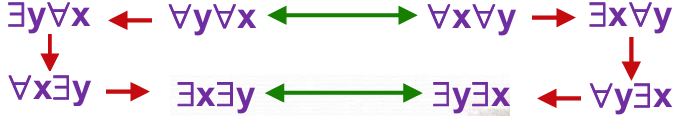
\includegraphics[width=0.8\linewidth]{image01}
	\label{fig:image01}
\end{figurehere}


4. 量词的消去/引入规则:
设 $x, y$ 为个体变元符号,$c$ 为个体常元,【$y$ 不在 $A(x)$ 中约束出现】
\begin{enumerate}
	\item \textbf{$\forall -$}:$(\forall x) A(x) \Rightarrow A(y), (\forall x) A(x) \Rightarrow A(c)$
	\item \textbf{$\forall +$}:$A(y) \Rightarrow (\forall x) A(x)$ 限制:$x$ 不在 $A(y)$ 中约束出现[重名引起混乱]
	\item \textbf{$\exists -$}:$(\exists x) A(x) \Rightarrow A(c)$ 限制:$(\exists x) A(x)$ 中无自由变元[否则$x$依赖于自由变元],且不含 $c$
	\item \textbf{$\exists +$}:$A(c) \Rightarrow (\exists x) A(x)$ 限制:$x$ 不出现于 $A(c)$
\end{enumerate}

\textbf{一阶自然推理系统$N_L$构造推理的证明}:\\
\fontsize{5.9pt}{6pt}
·推理规则:$12$条命题逻辑推理规则、$\forall -, \forall +, \exists -, \exists +$\\
\fontsize{6pt}{7pt}
·推理方法:\\
1. 前提引入规则和结论引入规则\\
2. 如果结论是以蕴涵形式(或析取形式)给出,可使用附加前提证明法\\
3. 若需消去量词,用全称量词消去规则和存在量词消去规则\\
4. 当所要求的结论可能被定量时,用全称量词引入规则和存在量词引入规则将量词加入\\
5. 对消去量词的公式或公式中不含量词的子公式,用命题演算中的基本等价公式和基本推理定律\\
6. 对含有量词的公式可以用谓词中的基本等价公式和基本推理定律

注1.如公式中既要消去存在量词又要消去全称量词,且所选用的个体是同一个符号,则必须 \textbf{先消去存在量词再消去全称量词}

\begin{figurehere}
	\centering
	
\includegraphics[width=0.7\linewidth]{image02}
	\label{fig:image02}
\end{figurehere}

注3.有两个含有存在量词的公式,当消去存在量词时,不能选用同样的一个常量符号来取代两个公式中的变元,而 \textbf{应用不同的常量符号}

注4.使用 $\forall +, \forall -, \exists +, \exists -$ 时,此量词必须位于整个公式的最前端,且它的辖域为其后的整个公式

\newpage
	\setlength{\abovedisplayskip}{0em}
	\setlength{\belowdisplayskip}{0em}
	
	\section*{集合基础概念}
	\textbf{子集}:$B \subseteq A \Leftrightarrow \forall x (x \in B \rightarrow x \in A)$
	
	\textbf{非子集}:$B \nsubseteq A \Leftrightarrow \exists x (x \in B \land x \notin A)$
	
	\textbf{相等}:$A = B \Leftrightarrow \forall x (x \in B \leftrightarrow x \in A) \Leftrightarrow A \subseteq B \land B \subseteq A$
	
	\textbf{真子集}:$A \subset B \Leftrightarrow A \subseteq B \land A \neq B$
	
	\textbf{非真子集}:$A \not\subset B \Leftrightarrow \exists x (x \in A \land x \notin B) \lor A = B$
	
	\textbf{空集}:$\emptyset = \{x | x \neq x\}$,是一切集合的子集;唯一
	
	\textbf{全集$E$}:与具体问题相关,不唯一
	
	\textbf{幂集}:$P(A) = 2^{A} = \{x | x \subseteq A\}$,易知$|P(A)| = 2^n$
	
	\textbf{n元集}:A有n个元素,记作$|A| = n$
	
	\textbf{有穷集(有限集)}:A的元素个数有限
	
	\textbf{并集}:$A \cup B = \{x | x \in A \lor x \in B\}$
	
	\textbf{初级并}:$A_1 \cup A_2 \cup \ldots \cup A_n = \{x | \exists i (1 \leq i \leq n \land x \in A_i)\}$,$\bigcup_{i=1}^n A_i = A_1 \cup A_2 \cup \ldots \cup A_n$,$\bigcup_{i=1}^\infty A_i = A_1 \cup A_2 \cup \ldots$
	
	\textbf{交集}:$A \cap B = \{x | x \in A \land x \in B\}$
	
	\textbf{初级交}:$A_1 \cap A_2 \cap \ldots \cap A_n = \{x | \forall i (1 \leq i \leq n \rightarrow x \in A_i)\}$,$\bigcap_{i=1}^n A_i = A_1 \cap A_2 \cap \ldots$,$\bigcap_{i=1}^\infty A_i = A_1 \cap A_2 \cap \ldots$
	
	\textbf{不相交}:设 $A_1, A_2, \ldots$ 是可数多个集合,对于任意的 $i \neq j$,都有 $A_i \cap A_j = \emptyset$,则称 $A_1, A_2, \ldots$ 是互不相交的
	
	\textbf{相对补集}:只属于 $A$ 而不属于 $B$ 的全体元素组成的集合为 $B$ 对 $A$ 的相对补集。$A - B = \{x | x \in A \land x \notin B\} = A \cap \sim B$
	
	\textbf{对称差}:$A \bigoplus B = \{x | (x \in A \land x \notin B) \lor (x \notin A \land x \in B)\} = (A - B) \cup (B - A) = (A \cup B) - (A \cap B)$
		
	\textbf{绝对补集}:$\sim A = \{x | x \in E \land x \notin A\} = E - A = \{x | x \notin A\}$
	
	\textbf{广义并}:$\bigcup A = \{x | \exists z (x \in z \land z \in A)\}$, $A$是集族(即A的元素是集合);$\bigcup \emptyset = \emptyset$
	
	\textbf{广义交}:$\bigcap A = \{x | \forall z (z \in A \rightarrow x \in z)\}$, $A$是集族且\textbf{非空}——理论上$\bigcap \emptyset$包含任意元素,即包含所有集合,这在集合论中无意义\\
	·$\{x | \forall z (z \in A \rightarrow x \in P(z))\}=\cap\{P(z)|z\in A\}$
	
	\textbf{集合运算的优先级}:一元运算优先于二元运算
	
	·第一类运算/一元运算(从右向左):\textbf{绝对补、幂集、广义交/并}
	
	·第二类运算/二元运算(从左向右):\textbf{初级并/交、相对补、对称差}
	
	\section*{二元关系}
	\textbf{有序对}:由两个元素 $x$ 和 $y$ (允许 $x = y$) 按照一定顺序排列而成的二元组称作一个有序对,记作 $\langle x, y \rangle := \{\{a\}, \{a, b\}\}$
	
	·$x \neq y \Rightarrow \langle x, y \rangle \neq \langle y, x \rangle$\\
	·$\langle a, b \rangle = \langle c, d \rangle \Leftrightarrow a = c \land b = d$
	
	\textbf{笛卡尔积(卡式积)}:设 $A, B$ 为集合,用 $A$ 中元素为第一元素,$B$ 中元素为第二元素构成有序对。所有这样的有序对组成的集合称作 $A$ 和 $B$ 的笛卡尔积,记作 $A \times B:=\{ \langle x, y \rangle | x \in A \land y \in B \}$
	
	\textbf{笛卡尔积性质}\\
	·非交换$A \times B \neq B \times A$【除非$A = \emptyset \lor B = \emptyset \lor A = B$】\\	
	·非结合$(A \times B) \times C \neq A \times (B \times C)$【除非$A = \emptyset \lor B = \emptyset \lor C = \emptyset$】\\	
	·对并和交满足分配律:
	\begin{itemize}
		\item[·] $A \times (B \cup C) = (A \times B) \cup (A \times C)$
		\item[·] $(B \cup C) \times A = (B \times A) \cup (C \times A)$
		\item[·] $A \times (B \cap C) = (A \times B) \cap (A \times C)$
		\item[·] $(B \cap C) \times A = (B \times A) \cap (C \times A)$
	\end{itemize}

	·$A \times \emptyset = \emptyset, \emptyset \times A = \emptyset$\\
	·$A \times B = \emptyset \Leftrightarrow A = \emptyset \lor B = \emptyset$\\
	·若 $A \neq \emptyset$, 则 $A \times B \subseteq A \times C \Leftrightarrow B \subseteq C$\\
	·$A \subseteq C \land B \subseteq D \Rightarrow A \times B \subseteq C \times D$【当$(A = B = \emptyset) \lor (A \neq \emptyset \land B \neq \emptyset)$ 时,逆命题成立】
	
	\textbf{n元关系}:元素全是有序n元组【或为空集】的集合\\
	\textbf{二元关系(关系)}:$n=2$的情形,记作 $R$\\
	·记号:$\langle x, y \rangle \in R \Leftrightarrow R(x,y), Rxy \Leftrightarrow x R y$\\
	·若 $\langle x, y \rangle \notin R$,记作 $x \not\sim R y$。
	
	\textbf{A到B的二元关系}:$A \times B$ 的任何子集(含空集)$\Leftrightarrow \quad R \subseteq A \times B \quad \Leftrightarrow \quad R \in \mathcal{P}(A \times B)$\\
	·$A$到$B$不同的二元关系有$2^{|A|\cdot|B|}$个\\
	·当 $A = B$ 时称作 $A$ 上的二元关系
	
	\textbf{特殊关系}:对于任何集合 $A$:\\
	·\textbf{空关系}:$\emptyset$ \\
	·\textbf{全域关系}:$E_A = \{ \langle x, y \rangle | x \in A \land y \in A \} = A \times A$ \\
	·\textbf{恒等关系}:$I_A = \{ \langle x, x \rangle | x \in A \}$ \\
	·\textbf{小于等于关系}:$LE_A = \{ \langle x, y \rangle | x, y \in A, x \leq y \}$ \\
	·\textbf{整除关系}:$D_A = \{ \langle x, y \rangle | x, y \in A, x | y \}$ \\
	·\textbf{包含关系}:$R_{\subseteq} = \{ \langle x, y \rangle | x, y \in A, x \subseteq y\}$\\
	·\textbf{真包含关系}:$R_{\subset} = \{ \langle x, y \rangle | x, y \in A, x \subset y\}$
		
	\textbf{关系矩阵}:$M(R)=[r_{ij}]_{n\times n}$,若 $x_i$ 与 $x_j$ 有关系则 $r_{ij}$ 为 1,否则为 0。
	
	\textbf{关系图}:$\langle x_i, x_j \rangle \in R$对应图 $G_R$ 中$x_i$ 到 $x_j$ 的有向边
	
	·集合表达式、关系矩阵、关系图三者可唯一互相确定。
	
	\textbf{逆关系}:$R^{-1} = \{ \langle x, y \rangle \mid \langle y, x \rangle \in R \}$\\
	\textbf{右复合}:$F \circ G = \{ \langle x, y \rangle \mid \exists t (\langle x, t \rangle \in F \land \langle t, y \rangle \in G) \}$
	
	\textbf{定义域}:$R$ 中所有有序对的第一元素构成的集合称作 $R$ 的定义域,记作 $\text{dom} R$,即 $\text{dom} R = \{ x \mid \exists y (\langle x, y \rangle \in R) \}$\\
	\textbf{值域}:$R$ 中所有有序对的第二元素构成的集合称作 $R$ 的值域,记作 $\text{ran} R$,即 $\text{ran} R = \{ y \mid \exists x (\langle x, y \rangle \in R) \}$\\
	\textbf{域}:$R$ 的定义域和值域的并集为域,记作 $\text{fld} R$,即 $\text{fld} R = \text{dom} R \cup \text{ran} R$
	
	\textbf{限制}:$R$ 在 $A$ 上的限制记作 $R \uparrow A$,即 $R \uparrow A = \{ \langle x, y \rangle \mid x R y \land x \in A \} \subseteq R$\\
	\textbf{像}:$A$ 在 $R$ 上的像记作 $R[A]$,即 $R[A] = \text{ran}(R \uparrow A) = \{ y \mid \exists x (x \in A \land x F y) \} \subseteq \text{ran} R$
	
	\textbf{幂运算}:$R$的$n$次幂
	\begin{itemize}
		\item[·] $R^0 = \{ \langle x, x \rangle \mid x \in A \} = I_A$
		\item[·] $R^{n+1} = R^n \circ R$
	\end{itemize}
	
	\textbf{关系运算的顺序}\\
	·逆运算优先于其他运算\\
	·关系运算(逆、合成、限制、像)优先于集合运算(交并补、相对补、对称差等)\\
	·没有规定优先权的运算以括号决定运算顺序
	
	\textbf{自反}:设 $R$ 为 $A$ 上的关系,$R$ 在 $A$ 上是自反的 $\Leftrightarrow \forall x (x \in A \rightarrow \langle x, x \rangle \in R) \Leftrightarrow (\forall x \in A) xRx$\\
	\textbf{非自反}:自反的否定,定义空关系非自反\\
	\textbf{反自反}:称 $R$ 在 $A$ 上是反自反的,若 $\forall x (x \in A \rightarrow \langle x, x \rangle \notin R)$
	
	\textbf{对称}:若 $\forall x \forall y (x, y \in A \land \langle x, y \rangle \in R \to \langle y, x \rangle \in R)$,则称 $R$ 为 $A$ 上对称的关系\\
	\textbf{反对称}:若 $\forall x \forall y (x, y \in A \land \langle x, y \rangle \in R \land \langle y, x \rangle \in R \to x=y)$,则称 $R$ 为 $A$ 上反对称的关系
	
	\textbf{传递}:$\forall x \forall y \forall z (x, y, z \in A \land \langle x, y \rangle \in R \land \langle y, z \rangle \in R \to \langle x, z \rangle \in R)$【若两步能到,一步一定能到】
	
	\textbf{自反/对称/传递闭包}:要求 $A$ 非空,$R$ 的$××$闭包是 $A$ 上的关系 $R'$满足$R \subseteq R'$、$××$性、极小性;分别记作$r(R), s(R), t(R)$\\
	·极小性的表示:$\forall S ((R \subseteq S \land S \text{自反}) \rightarrow r(R) \subseteq S)$
	
	\textbf{等价关系}:设 $R$ 为非空集合 $A$ 上的关系,若 $R$ 是自反、对称、传递的,则称 $R$ 为 $A \text{上的等价关系}$\\
	·设 $R$ 为一个等价关系,若 $\langle x, y \rangle \in R$,则称 $x$ 等价于 $y$,记作 $x \sim y$。空关系不是等价关系。
	
	\textbf{等价类}:设 $R$ 为非空集合 $A$ 上的等价关系,$\forall x \in A$,令 $[x]_R = \{ y \mid y \in A \land x R y \}$,称 $[x]_R$ 为 $x$ 关于 $R$ 的等价类,简记为 $[x]$
	
	\textbf{商集}:设 $R$ 为非空集合 $A$ 上的等价关系,$R$ 的所有等价类组成的集合是 $A$ 关于 $R$ 的商集,记作 $A/R$,即$A/R = \{ [x]_R \mid x \in A \} \quad \text{(是一个集族)}$\\
	·显然$\cup A/R=A$
	
	\textbf{划分}:$A \neq \emptyset$ 的一个划分是 $A$ 的子集族 $\mathcal{A} \subseteq P(A)$ 满足:$\emptyset \notin \mathcal{A},~ \forall x \forall y (x, y \in \mathcal{A} \land x \neq y \to x \cap y = \emptyset),~ \bigcup \mathcal{A} = A$,称 $\mathcal{A}$ 中的元素为 $A$ 的划分块。\\	
	·$R$\text{是}$A$ 上的等价关系 $\Rightarrow$ 商集 $A/R$ 是 $A$ 的划分\\
	·$\mathcal{A}$\text{是}$A$\text{的划分}$\Leftrightarrow$\text{同块关系} $R_{\mathcal{A}}$是$A$上的等价关系\\	
	·注:求所有等价关系时并上$I_A$(自反性)
	
	\textbf{Stirling\text{子集数}}:记$f[n][k]$\text{为}n个不同元素划分为k组的方法数, $f[n][0]=0, f[n][1]=1, f[n][2]=2^{n-1}-1, f[n][n-1]=C^2_n, f[n][n]=1, f[n][k]=kf[n-1][k]+f[n-1][k-1]$\\
	·$\Sigma f[3][k]=5, \Sigma f[4][k]=15$
	
	\textbf{偏序关系}:设 $A \neq \varnothing, R \subseteq A \times A$,若 $R$ 是自反、反对称、传递的,则称 $R$ 为 $A$ 的偏序关系,记作 $\preccurlyeq$。设 $\preccurlyeq$ 为偏序关系,如果 $\langle x, y \rangle \in \preccurlyeq$,则记作 $x \preccurlyeq y$\\
	·自反时证反对称:$xRy \land yRx \Rightarrow x=y$
	
	\textbf{偏序集}:$\preccurlyeq$\text{是}$A$上的偏序关系,称 $\langle A, \preccurlyeq \rangle$为偏序集
	
	设  $\langle A, \preccurlyeq \rangle$为偏序集,$x, y \in A$,定义:\\	
	·$x$\text{与}$y$\textbf{可比}:若$x \preccurlyeq y \lor y \preccurlyeq x$\\
	·\textbf{严格小于}:$x \prec y \Leftrightarrow x \preccurlyeq y \land x \neq y$\\
	·\textbf{覆盖}:称$y$覆盖$x$,若 $x \prec y$,且不存在 $z$,使得 $x \prec z \prec y$\\
	·对任意两个元素 $x, y$,有四种情况必发生其中恰好一种:$x \prec y$,$y \prec x$,$x = y$,$x$ 与 $y$ 不是可比的
	
	\textbf{哈斯图}:$\forall x, y \in A$,若 $x \prec y$,则将 $x$ 画在 $y$ 下方;对于 $A$ 中两个不同的元素 $x$ 和 $y$,若 $y$ 覆盖 $x$,就用一条线段连接 $x$ 和 $y$\\
	·省略自反性、传递性及反对称性的箭头
	
	\textbf{全序关系(线序关系)}:设 $\langle A, \preccurlyeq \rangle$ 为偏序集,若 $\forall x, y \in A$,$x$ 与 $y$ 都是可比的,则 $R$ 为 $A$ 上的全序关系(哈斯图是一根线)
	
	\textbf{拟序关系}:设 $R$ 为非空集合 $A$ 上的关系。若 $R$ 是反自反、传递的,则称 $R$ 为 $A$ 上的拟序关系,常用 $\prec$ 表示拟序关系,$\langle A, \prec \rangle$ 为拟序集。\\
	·反自反性与传递性蕴涵反对称性
	
	\textbf{最/极大/小元}:设 $\langle A, \preccurlyeq \rangle$ 为偏序集,$B \subseteq A, y \in B$
	\begin{itemize}
		\item[·] 若 $\forall x (x \in B \to y \preccurlyeq x)$成立,则称$y$\text{为}$B$ 的最小元【可以无必唯一】
		\item[·] 若 $\forall x (x \in B \land x \preccurlyeq y \to x = y)$\text{成立,则称}$y$\text{为}$B$ 的极小元【必存在不唯一,不大于任何元】
	\end{itemize}
	
	\textbf{上/下界}:设 $\langle A, \preccurlyeq \rangle$ 为偏序集,$B \subseteq A, y \in A$
	\begin{itemize}
		\item[·] 若 $\forall x (x \in B \to x \preccurlyeq y)$ 成立,则称 $y$\text{为}$B$ 的上界【可以无不唯一】
		\item[·] 令 $C = \{ y \mid y \text{为} B \text{的上界} \}$,则称 $C$ 的最小元为 $B$ 的最小上界或上确界【可以无必唯一】
		\item[·] 上界与下界不一定存在集合之中
		\item[·] 集合的最小元素是它的下确界,最大元素就是它的上确界;反之不对
	\end{itemize}
	
	\textbf{函数(映射)}:单值的二元关系$F$,若 $\forall x \in \text{dom} F$ 都存在唯一的 $y \in \text{ran} F$ 使得 $xFy$ 成立(单值)\\
	·记号:$F(x) = y \Leftrightarrow \langle x, y \rangle \in F \Leftrightarrow x F y$\\
	·证单值:$\forall x \in \text{dom} F, \forall y, z \in \text{ran} F, x F y \land x F z \rightarrow y = z$
	
	\textbf{偏函数(部分函数)}:若 $\text{dom} F \subseteq A \land \text{ran} F \subseteq B$,则 $F$ 称为从 $A$ 到 $B$ 的偏函数,$A$ 称为 $F$ 的前域,$B$ 称为 $F$ 的后域,记作\\
	·\textbf{偏函数计数}:$(|B|+1)^{|A|}$
	
	\textbf{全函数(函数)}:若 $\text{dom} f = A \land \text{ran} f \subseteq B$,则 $f$ 称为从 $A$ 到 $B$ 的函数,记作 $f: A \rightarrow B$\\
	·所有从 $A$ 到 $B$ 的函数的集合记作 $B^A$,读作“$B$ 上 $A$”;$B^A = \{ f \mid f: A \rightarrow B \}$;$|B^A| = |B|^{|A|}$\\
	·当 $A = \emptyset$ 时,$B^A = \{ \emptyset \}$,$|B^A| = 1$\\
	·当 $A \neq \emptyset \land B = \emptyset$ 时,$B^A = \emptyset$,$|B^A| = 0$
		
	\textbf{单射、满射、双射}:设 $f: A \rightarrow B$
	\begin{itemize}
		\item[·] 若 $\text{ran} f = B$,则称 $f$ 为满射
		\item[·] 若 $\forall y \in \text{ran} f$ 都存在唯一的 $x \in A$ 使得 $f(x) = y$,则称 $f$ 为单射
		\item[·] 若 $f$ 既单射又满射,则 $f$ 为双射(一一对应)
	\end{itemize}
	\textbf{单射、满射、双射计数}:设$|A|=n, |B|=m$
	\begin{itemize}
		\item[·] $n<m$时,单射个数$m!/(m-n)!$
		\item[·] $n>m$时,满射个数$m!f[n][m]$
		\item[·] $n=m$时,单/满/双射个数$n!$
	\end{itemize}
	
	\textbf{常数函数} 设 $f: A \rightarrow B$,若存在 $c \in B$ 使得对所有 $x \in A$ 都有 $f(x) = c$,则称 $f$ 为常数函数\\
	\textbf{恒等函数}:称 $A$ 上的恒等关系 $I_A: A\rightarrow A$ 为 $A$ 上的恒等函数,$I_A(x) = x$\\
	\textbf{特征函数}:$A$ 的特征函数 $\chi_{A}: E \rightarrow \{0, 1\}$ 定义为$\chi_{A}(x) = 1\text{ if } a \in A$,否则为$0$\\
	·当 $\emptyset \subset A \subset E$ 时,$\chi_{A}$ 是满射
	
	\textbf{单调函数}:\text{设}$\langle A, \leqslant_A \rangle, \langle B, \leqslant_B
	 \rangle$ 为偏序集,$f: A \rightarrow B$,若$\forall x_1, x_2 \in A$,$x_1 \leqslant_A x_2 \Rightarrow f(x_1) \leqslant_B f(x_2)$,则称 $f$单调递增\\
	·\text{严格单调}:\text{把}$\leqslant$\text{换成}$<$,要求$f$是单射
	
	
	\textbf{自然映射(典型映射)}:设 $R$ 是 $A$ 上的等价关系,令 $f: A \rightarrow A/R$,$f(x) = [x]_R, \forall a \in A$,称 $f$ 是从 $A$ 到商集 $A/R$ 的自然映射\\
	·不同的等价关系确定不同的自然映射,恒等关系确定的是双射,其他自然映射一般只是满射
	
	\hrule
	
	\section*{计数问题}	
	
	\textbf{文氏图}:大矩形表示全集 $E$(可省略),在矩形内部画圆,用圆或其他闭曲线的内部表示集合。不同的圆代表不同的集合,并将运算结果得到的集合用阴影部分表示——计数问题:
	
	1. 画文氏图,一般每个集合对应一种性质
	
	2. 计算各区域的数量,有未知的则列方程
	
	\textbf{包含排斥原理(容斥原理)} 设 $A_1, A_2, \ldots, A_n$ 为 $n$ 个集合,则
	\fontsize{4pt}{4pt}
	\begin{equation*}
		\left| \bigcup_{i=1}^{n} A_i \right| = \sum_{i=1}^{n} |A_i| - \sum_{i<j}|A_i \cap A_j| + \sum_{i<j<k}|A_i \cap A_j \cap A_k| - \cdots + (-1)^{n-1}|A_1 \cap A_2 \cap \cdots \cap A_n|
	\end{equation*}
	\fontsize{6pt}{6pt}
	
	\section*{集合恒等式}	
	
	\textbf{幂等律} $A \cup A = A$,$A \cap A = A$
	
	\textbf{交换律} $A \cup B = B \cup A$,$A \cap B = B \cap A$
	
	\textbf{结合律} $(A \cup B) \cup C = A \cup (B \cup C)$,$(A \cap B) \cap C = A \cap (B \cap C)$
	
	\textbf{分配律} $A \cup (B \cap C) = (A \cup B) \cap (A \cup C)$,$A \cap (B \cup C) = (A \cap B) \cup (A \cap C)$
	
	\textbf{德摩根律} 
	
	相对形式:$E - (A \cup B) = (E - A) \cap (E - B)$,$E - (A \cap B) = (E - A) \cup (E - B)$
	
	绝对形式:$\sim(A \cup B) = \sim A \cap \sim B$,$\sim(A \cap B) = \sim A \cup \sim B$
		
	\textbf{吸收律} $A \cup (A \cap B) = A$,$A \cap (A \cup B) = A$
	
	\textbf{零律} $A \cup E = E$,$A \cap \emptyset = \emptyset$
	
	\textbf{同一律} $A \cup \emptyset = A$,$A \cap E = A$
		
	\textbf{排中律} $A \cup \sim A = E$
	
	\textbf{矛盾律} $A \cap \sim A = \emptyset$
		
	\textbf{余补律} $\sim \emptyset = E$,$\sim E = \emptyset$
	
	\textbf{双重否定律} $\sim(\sim A) = A$
	
	\textbf{补交转换律} $A - B = A \cap \sim B$(消去差集运算符)
	
	对于集合定律的证明应该使用数理逻辑

	\textbf{子集的性质}
	\begin{itemize}
		\item[·] $A \subseteq B \Rightarrow (A \cup C) \subseteq (B \cup C)$
		\item[·] $A \subseteq B \Rightarrow (A \cap C) \subseteq (B \cap C)$
		\item[·] $(A \subseteq B) \wedge (C \subseteq D) \Rightarrow (A \cup C) \subseteq (B \cup D)$
		\item[·] $(A \subseteq B) \vee (C \subseteq D) \Rightarrow (A \cap C) \subseteq (B \cap D)$
		\item[·] $(A \subseteq B) \wedge (C \subseteq D) \Rightarrow (A - C) \subseteq (B - D)$
		\item[·] $C \subseteq D \Rightarrow (A - D) \subseteq (A - C)$
	\end{itemize}
	
	\textbf{差集的性质}
	\begin{itemize}
		\item[·] $A - B = A - (A \cap B)$
		\item[·] $A - B = A \cap \sim B$
		\item[·] $A \cup (B - A) = A \cup B$
		\item[·] $A \cap (B - C) = (A \cap B) - C$
	\end{itemize}
	
	\textbf{对称差的性质}
	\begin{itemize}
		\item[·] 交换律,结合律
		\item[·] 分配律:$A \cap (B \bigoplus C) = (A \cap B) \bigoplus (A \cap C)$
		\item[·] ~~~~~:$A \bigoplus (A \bigoplus B) = B$
		\item[·] 同一律:$A \bigoplus \emptyset = A$
		\item[·] 零律:$A \bigoplus A = \emptyset$
	\end{itemize}
	
	\textbf{幂集的性质}
	\begin{itemize}
		\item[·] $A \subseteq B \Leftrightarrow P(A) \subseteq P(B)$
		\item[·] $A = B \Leftrightarrow P(A) = P(B)$
		\item[·] $P(A) \in P(B) \Rightarrow A \in B$
		\item[·] $P(A) \cap P(B) = P(A \cap B)$
		\item[·] $P(A) \cup P(B) \subseteq P(A \cup B)$
		\item[·] $P(A - B) \subseteq (P(A) - P(B)) \cup \{\emptyset\}$
		\item[·] $A \subseteq P(A)$; $\cup P(A) = A$
		\item[·] $\{x\} \in P(A) \Leftrightarrow x \in A$
		\item[·] $x \in P(A) \Leftrightarrow x \subseteq A$
	\end{itemize}
	
	\section*{关系的运算}
	\textbf{基本运算}:
	\begin{itemize}
		\item[·] $R \cup S = \{ \langle x, y \rangle \mid x R y \lor x S y \}$
		\item[·] $R \cap S = \{ \langle x, y \rangle \mid x R y \land x S y \}$
		\item[·] 相对补$R - S = \{ \langle x, y \rangle \mid x R y \land x \cancel{S} y \}$
		\item[·] 绝对补$\sim R = A \times B - R$
	\end{itemize}

	\textbf{逆}:
	\begin{itemize}
		\item[·] $(F^{-1})^{-1} = F$
		\item[·] $\text{dom} F^{-1} = \text{ran} F, \text{ran} F^{-1} = \text{dom} F$
		\item[·] $M(R^{-1}) = (M(R))^T$
	\end{itemize}
	
	\textbf{合成(复合)}:
	\begin{itemize}
		\item[·] 结合律:$(F \circ G) \circ H = F \circ (G \circ H)$
		\item[·] $(F \circ G)^{-1} = G^{-1} \circ F^{-1}$
		\item[·] $M(R_1 \circ R_2) = M(R_1) \cdot M(R_2)$
	\end{itemize}
	
	\textbf{恒等关系性质}:$R \circ I_A = I_A \circ R = R$
	
	\textbf{仅并的复合有分配律}:本质$\exists$与$\land, \lor$的关系
	\begin{itemize}
		\item[·] $F \circ (G \cup H) = F \circ G \cup F \circ H$
		\item[·] $(G \cup H) \circ F = G \circ F \cup H \circ F$
		\item[·] $F \circ (G \cap H) \subseteq F \circ G \cap F \circ H$【注意是子集】
		\item[·] $(G \cap H) \circ F \subseteq G \circ F \cap H \circ F$【注意是子集】
	\end{itemize}
	
	\textbf{限制和像与交并的性质}:
	\begin{itemize}
		\item[·] $F \uparrow (A \cup B) = F \uparrow A \cup F \uparrow B$
		\item[·] $F[A \cup B] = F[A] \cup F[B]$
		\item[·] $F \uparrow (A \cap B) = F \uparrow A \cap F \uparrow B$
		\item[·] $F[A \cap B] \subseteq F[A] \cap F[B]$
		\item[·] $F[A] - F[B] \subseteq F[A - B]$
	\end{itemize}
	
	\textbf{幂运算}:\\
	·设 $A$ 为 $n$ 元集,$R$ 是 $A$ 上的关系,则$\exists s,t\in \mathbb{N} \text{使得}R^s = R^t$;因为A上一共只有$2^{n^2}$种关系
	\begin{itemize}
		\item[·] 对任何 $k \in \mathbb{N}$ 有 $R^{s+k} = R^{t+k}$
		\item[·] 对任何 $k, i \in \mathbb{N}$ 有 $R^{s + kp + i} = R^{s + i}$,其中 $p = t - s$
		\item[·] 令 $S = \{R^0, R^1, \ldots, R^{t-1}\}$,则对任意的 $q \in \mathbb{N}$ 有 $R^q \in S$
	\end{itemize}
	
	·设 $R$ 为 $A$ 上的关系,$m, n \in \mathbb{N}$,则:
	\begin{itemize}
		\item[·] $R^m \circ R^n = R^{m+n}$
		\item[·] $(R^m)^n = R^{mn}$
	\end{itemize}
		
	\textbf{关系性质的充要条件}:	设 $R$ 为 $A$ 上的关系,则
	\vspace{-10pt}
	\begin{center}
		\begin{tabular}{|@{\hskip 0pt}>{\centering\arraybackslash}p{14pt}@{\hskip 0pt}|@{\hskip 0pt}>{\centering\arraybackslash}p{15pt}@{\hskip 0pt}|@{\hskip 0pt}>{\centering\arraybackslash}p{20pt}@{\hskip 0pt}|@{\hskip 0pt}>{\centering\arraybackslash}p{25pt}@{\hskip 0pt}|@{\hskip 0pt}>{\centering\arraybackslash}p{26pt}@{\hskip 0pt}|@{\hskip 0pt}>{\centering\arraybackslash}p{30pt}@{\hskip 0pt}|}
			\hline
			 & 自反 & 反自反 & 对称性 & 反对称性 & 传递性 \\
			\hline
			集式 & $I_A \subseteq R$ & $R \cap I_A = \emptyset$ & $R = R^{-1}$ & $R \cap R^{-1} \subseteq I_A$ & $R \circ R \subseteq R$ \\
			\hline
			关系矩阵$M(R)$ & $M_{ii}=1$ & $M_{ii}=0$ & $M^T=M$ & 对 $i \neq j$,$M_{ji}+M_{ij} \leqslant 1$ &  $M^2_{ij} \leqslant M_{ij}$ \\
			\hline
			关系图$G(R)$ & 每个顶点都有环 & 每个顶点都没有环 & 相异点有一对方向相反的边或者没边 & 相异点仅有一条单向边或者没边 & 若$ab, bc$间都有边,则$ac$间有边 \\
			\hline
		\end{tabular}
	\end{center}
	\vspace{-5pt}
	·对称性与反对称性可以同时拥有(即仅有环)\\
	·自反性与反自反性不可以同时拥有(除非定义在空集上的空关系)
	
	\textbf{$R_1, R_2 \subseteq A \times A$ 具有某些共同性质,经过运算后保留原性质如下表:}\\
	\vspace{-10pt}
	\begin{center}
		\resizebox{130pt}{!}{ % 自动调整宽度
			\begin{tabular}{|c|c|c|c|c|c|}
				\hline
				表达式                          & 自反  & 反自反 & 对称  & 反对称 & 传递  \\
				\hline
				$R_1^{-1}, R_2^{-1}$          & \ding{51}   & \ding{51}   & \ding{51}   & \ding{51}   & \ding{51}   \\
				\hline
				$R_1 \cup R_2$                & \ding{51}   & \ding{51}   & \ding{51}   &     &     \\
				\hline
				$R_1 \cap R_2$                & \ding{51}   & \ding{51}   & \ding{51}   & \ding{51}   & \ding{51}   \\
				\hline
				$R_1 \circ R_2, R_2 \circ R_1$ & \ding{51}   &     &     &     &     \\
				\hline
				$R_1 - R_2, R_2 - R_1$        &     & \ding{51}   & \ding{51}   & \ding{51}   &     \\
				\hline
				$\sim R_1, \sim R_2$          &     &     & \ding{51}   &     &     \\
				\hline
			\end{tabular}
		}
	\end{center}
	
	\textbf{闭包的求法}:
	设 $R$ 为 $A$ 上的关系,则有:
	\begin{itemize}
		\item[·] $r(R) = R \cup I_A$
		\item[·] $s(R) = R \cup R^{-1}$
		\item[·] $t(R) = R \cup R^2 \cup R^3 \cup \cdots$
	\end{itemize}
	
	\textbf{引理}:$(R_1 \cup R_2)^{-1} = R_1^{-1} \cup R_2^{-1}$\\	
	\textbf{引理}:$(R_1 \cup R_2)^{2} = R_1^{2} \cup (A \circ B) \cup (B \circ A) \cup R_2^{2}$
	
	关系矩阵求闭包:$M_r = M \lor E, M_s = M \lor M^T, M_t = M \lor M^2 \lor M^3 + \cdots$
	
	关系图求闭包:
	\begin{itemize}
		\item[·] 自反闭包:每一个顶点没有环就加上一个环
		\item[·] 对称闭包:每一条边没有反向边就加上反向边
		\item[·] 传递闭包:$A$到$B$可达,就加$A$到$B$的边
	\end{itemize}
	
	\textbf{闭包的性质}:
	设 $R$ 是非空集合 $A$ 上的关系,~则 $R$ 是自反的 $\Leftrightarrow r(R) = R$;$R$ 是对称的 $\Leftrightarrow s(R) = R$;$R$ 是传递的 $\Leftrightarrow t(R) = R$
	
	\textbf{闭包与包含关系}:
	$\text{若 } R_1 \subseteq R_2 \subseteq A \times A \text{ 且 } A \neq \emptyset, \text{ 则}$
	$r(R_1) \subseteq r(R_2)$;$s(R_1) \subseteq s(R_2)$;$t(R_1) \subseteq t(R_2)$
	
	证明步骤:
	\begin{enumerate}
		\item[·] $R_1 \subseteq R_2; R_2 \subseteq r(R_2) \Rightarrow R_1 \subseteq r(R_2)$
		\item[·] $r(R_2)$ 自反;$r(R_1)$ 定义可得 $r(R_1) \subseteq r(R_2)$
	\end{enumerate}
	
	\textbf{闭包与并}:设 $R_1, R_2 \subseteq A$,且 $A \neq \emptyset$,则:
	\begin{itemize}
		\item[·] $r(R_1 \cup R_2) = r(R_1) \cup r(R_2)$【自反的并自反】
		\item[·] $s(R_1 \cup R_2) = s(R_1) \cup s(R_2)$【对称的并对称】
		\item[·] $t(R_1 \cup R_2) \supseteq t(R_1) \cup t(R_2)$【传递并未必传递】
	\end{itemize}
	
	\textbf{闭包与关系性质}:注意对称与传递!
	\begin{itemize}
		\item[·] 若 $R$ 是自反的,则 $s(R), t(R)$ 是自反的
		\item[·] 若 $R$ 是对称的,则 $r(R), t(R)$ 是对称的
		\item[·] 若 $R$ 是传递的,则 $r(R)$ 是传递的
	\end{itemize}
	
	\textbf{反例}:$R\text{传递,但是} s(R) \text{ 非传递}: A=\{1,2\}, R=\{<1,2>\}$
	
	\textbf{引理}:$(R \cup I_A)^n = I_A \cup R \cup R^2 \cup \cdots \cup R^n \quad (n \geq 1)$
	
	\textbf{定理}:$sr(R) = rs(R), tr(R) = rt(R), st(R) \subseteq ts(R)$
	
	例:$tsr(R) = trs(R) = rts(R)$ 是等价关系
	
	$str(R) = srt(R) = rst(R)$ 不是,无传递性
	
	\textbf{等价关系性质}:$R \text{为非空集合} A \text{上的等价关系,则}$
	\begin{itemize}
		\item[·] $\forall x \in A$, $[x]_R \neq \emptyset$,因为$xRx$
		\item[·] $\forall x, y \in A$,$xRy \Rightarrow [x] = [y]$
		\item[·] $\forall x, y \in A$,$\lnot xRy \Rightarrow [x] \cap [y] = \emptyset$
		\item[·] $\cup \{[x] \mid x \in A\} = A$
	\end{itemize}
	
	\textbf{序关系性质}:设 $\preccurlyeq$ 是非空集合 $A$ 上偏序关系,$\prec$ 是 $A$ 上的拟序关系,则\\
	·$\prec$ 是反对称的\\
	·$\preccurlyeq-I_A$ 是 $A$ 上的拟序关系\\
	·$\prec\cup I_A$ 是 $A$ 上的偏序关系\\
	·若 $x \prec y, x = y, y \prec x$ 中至多有一成立\\
	·$(x \prec y \vee x = y) \wedge (y \prec x \vee y = x) \Rightarrow x = y$
	
	\section*{函数相关定理}
	
	\textbf{定理1}:
	设 $F:A \rightarrow B, G:B \rightarrow C$,则 $F \circ G:A \rightarrow C$ 也是函数,且 $F \circ G(x) = G(F(x))$\\
	·证:$F \circ G$单值;$\text{dom }F \circ G = A,  \text{ran } F\circ G \subseteq C$【$\subseteq$显然,$=$利用全函数定义】;$F \circ G(x) = G(F(x))$\\
	\textbf{推论1}:
	设 $F, G, H$ 是函数,有 $(F \circ G) \circ H = F \circ (G \circ H)$
	
	\textbf{定理2}:
	设 $f: A \rightarrow B, g: B \rightarrow C$:
	\begin{itemize}
		\item[·] 如果 $f,g$ 都是满射的,则 $f \circ g$ 也是满射的
		\item[·] 如果 $f,g$ 都是单射的,则 $f \circ g$ 也是单射的
		\item[·] 如果 $f,g$ 都是双射的,则 $f \circ g$ 也是双射的
		\item[·] 如果 $f \circ g$ 是满射的,则 $g$ 是满射
		\item[·] 如果 $f \circ g$ 是单射的,则 $f$ 是单射
		\item[·] 如果 $f \circ g$ 是双射的,则 $f$ 是单射,$g$ 是满射
	\end{itemize}
	
	\textbf{定理3}:
	设 $f: A \rightarrow B$,则有 $f = f \circ I_B = I_A \circ f$
	
	\textbf{定理4}:
	$f, g$ 都是单调增/都是单调减的,则 $f \circ g$ 是单调增的
	
	\textbf{定理5(反函数)}:
	设 $f: A \rightarrow B$ 是双射,则 $f^{-1}: B \rightarrow A$ 也是双射;且 $f^{-1} \circ f = I_B, f \circ f^{-1} = I_A$
\end{multicols*}
\end{document}